\documentclass[ngerman,12pt]{article}

% PACKAGES
\usepackage[ngerman]{babel}
\usepackage[utf8]{inputenc}
\usepackage{url}
\usepackage{a4}
\usepackage{amsfonts}
\usepackage{amsmath}
\usepackage[usenames,dvipsnames]{xcolor}
\usepackage{verbatim}
\usepackage{graphicx}
\usepackage[colorlinks=true]{hyperref}
\hypersetup{urlcolor=blue,
			linkcolor=blue,
			citecolor=blue}
\usepackage{listings}
\usepackage{booktabs}
\usepackage{caption}
\usepackage[babel, german=quotes]{csquotes}
\usepackage[backend = biber,style = alphabetic]{biblatex}
\addbibresource{literatur.bib}
\setlength{\bibitemsep}{1em}
\usepackage{multirow}



% PAGE LAYOUT
\setlength{\textwidth}{174mm}
\setlength{\textheight}{220mm}
\setlength{\topmargin}{10mm}
\setlength{\oddsidemargin}{10mm}
\setlength{\hoffset}{0mm}
\setlength{\voffset}{0mm}
\setlength{\parindent}{0mm}
\setlength{\parskip}{2mm}
\pagestyle{plain}

% EXERCISE SHEET SPECIFIC MAKROS
\renewcommand{\title}[1]{\par\vspace{5mm}\centerline{\Large #1}}
\newcommand{\subtitle}[1]{\par\vspace{1mm}\centerline{\footnotesize #1}\par}
\newcommand{\exercise}[1]{\par\vspace{3mm}{\bf Aufgabe{\hspace{1mm}}#1}\hspace{1mm}}
\definecolor{dark-gray}{gray}{0.40}
\newcommand{\TODO}[1]{{\sf\color{blue} [#1]}}
\usepackage{lmodern}

% GENERALLY USEFUL MATH MAKROS
\def\ceil#1{{\left\lceil#1\right\rceil}}
\def\floor#1{{\left\lfloor#1\right\rfloor}}
\def\mod{\mbox{ mod }}
\def\div{\mbox{ div }}
\def\sm{\backslash}
\def\IN{\mathbb{N}}
\def\IZ{\mathbb{Z}}
\def\IR{\mathbb{R}}
\def\Oh#1{O\left(#1\right)}
\def\Om#1{\Omega\left(#1\right)}
\def\Th#1{\Theta\left(#1\right)}
\def\eps{\varepsilon}

\begin{document}

% COLORS
\definecolor{darkblue}{rgb}{0.0,0.0,0.6}
\definecolor{darkred}{rgb}{0.7,0.0,0.0}

% HEAD OF EXERCISE SHEETS
\setlength{\textwidth}{16.5cm}
\setlength{\textheight}{22cm}
\setlength{\topmargin}{0cm}
\setlength{\oddsidemargin}{-0.3cm}
\setlength{\evensidemargin}{0cm}
\vspace*{-20mm}

% Links der Name des Lehrstuhls.
\parbox{20mm}{
~\\[0mm]
~\\[0mm]
~\\[-5mm]} %\\[0.3mm]
% In der Mitte der Name der Veranstaltung.
\parbox{120mm}{\vspace*{1mm}\begin{center}\large\bf%
Einführung in die Programmierung für Studierende der Naturwissenschaften\\[0mm]
\hspace{5mm} SS 2021\\[0mm]
{\footnotesize\rm \url{https://aam.uni-freiburg.de/agdo/lehre/ss21/prog/index.html}}%
\end{center}}
\par\vspace{-5mm}
% Grauer Strich und rechts das Uni-Logo.
\definecolor{freiburg-gray}{rgb}{0.68,0.68,0.68}
\vspace*{2mm}
\raisebox{1.19cm}{%
\textcolor{freiburg-gray}{\rule{0.885\textwidth}{1.1mm}}}
\par\vspace*{-37.84mm}
\hspace*{\fill}
\includegraphics[width=74pt,height=107pt]{Uni_Logo.png}
\par\vspace{-5mm}

\bigskip

\title{Codebreaker für Caesar-Verschlüsselung mit Häufigkeitsanalyse}
\subtitle{von Daniel Rath und Theresa Maurer}
\renewcommand{\baselinestretch}{1.1}\normalsize

\bigskip
\subsection*{Verschlüsselung und Entschlüsselung}
Die Caesar-Verschlüsselung ist eine einfache, monoalphabetische Verschlüsselung. Die Verschlüssel- ung der Buchstaben a - z entspricht einer Verschiebung des Alphabets um beliebig viele Stellen. Zwischen Groß- und Kleinbuchstaben wird nicht unterschieden.\cite{Beutelspacher2007}\\ 
Beispielsweise wird bei einer Verschiebung um drei Buchstaben das a auf das d abgebildet, das b wird auf das e abgebildet, das c wird auf das f abgebildet, für die anderen Buchstaben wird diese Verfahrensweise analog weitergeführt. Nach der Systematik der Chiffrierung wird die Verschiebung nach dem z beim a weitergeführt. Also wird das w auf das z abgebildet und das x folglich auf das a.

\begin{table}[ht]
\centering
\label{table:bspaisd}
\begin{tabular}{*{23}{|c}|}
	\hline
	\textbf{Klartext:} & a & b & c & d & e & f & \dots & l & m & n & o & p & q & r & s & t & u & v & w & x & y & z \\
	\hline
	\textbf{Chiffre:} & d & e & f & g & h & i & \dots & o & p & q & r & s & t & u & v & w & x & y & z & a & b & c \\
	\hline
	
\end{tabular}
%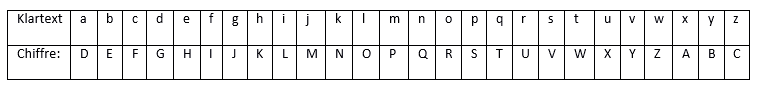
\includegraphics[width=520pt,height=60pt]{Beispiel c=3.png}
\captionof{table}{Beispiel für eine Caesar-Verschlüsselung mit Verschiebung um 3 Buchstaben}
\end{table}

Die Verschlüsselung eines Textes lässt sich bei der Programmierung leichter umsetzen, wenn jeder Buchstabe in seiner ASCII-Darstellung betrachtet wird. Das heißt jeder Buchstabe wird als Zahl dargestellt, die Verschiebung entspricht einer Addition. Eine Verschiebung um drei Buchstaben entspricht einer Addition mit der Zahl 3.

\newpage

Jedem Buchstaben des Alphabets ist eine Zahl im ASCII-Code zugeordnet:

\begin{table}[ht]
	\label{table:asciimaping}
	\centering
	\begin{tabular}{|r|c|r|c|r|c|}
		\hline
		\textbf{Buchstabe} & \textbf{ASCII} & \textbf{Buchstabe} & \textbf{ASCII} & \textbf{Zahl} & \textbf{ASCII}\\
		\hline
		A & 65 & a & 97 & 0 & 48\\
		\hline
		B & 66 & b & 98 & 1 & 49\\
		\hline
		C & 67 & c & 99 & 2 & 50\\
		\hline
		\multirow{3}{*}{\vdots} & \multirow{3}{*}{\vdots} & \multirow{3}{*}{\vdots} & \multirow{3}{*}{\vdots} &  \multirow{3}{*}{\vdots} & \multirow{3}{*}{\vdots}\\
		& & & & & \\
		& & & & & \\
		\hline
		J & 74 & j & 106 & 9 & 57\\
		\hline
		\multirow{3}{*}{\vdots} & \multirow{3}{*}{\vdots} & \multirow{3}{*}{\vdots} & \multirow{3}{*}{\vdots} &  & \\
		& & & & & \\
		& & & & & \\
		\hline
		X & 88 & x & 120 & &\\
		\hline
		Y & 89 & y & 121 & &\\
		\hline
		Z & 90 & z & 122 & &\\
		\hline
		
	\end{tabular}
\captionof{table}{Groß-/Kleinbuchstaben und Zahlen mit dem entsprechenden ASCII-Code \cite{Roitzsch1993}}
\end{table}

Der Einfachheit halber beschränken wir uns hier auf die Kleinbuchstaben von a-z, also die ASCII-Zeichen 97-122.
Ein Kleinbuchstabe x in ASCII-Darstellung kann nun durch eine additive Funktion 
\begin{equation*}
C(x)=((x - 97) + c) \mod 26) +97
\end{equation*}
verschlüsselt werden, für ein $c \in \mathbb{Z}$. Der verschlüsselte Buchstabe ist wieder eine Zahl zwischen 97-122 und somit auch ein Kleinbuchstabe. Das c bewirkt die Verschiebung des Alphabets.\\
Die zugehörige Dechiffrierfunktion ist 
\begin{equation*}
D(x)=((x - 97) - c) \mod 26) +97´
\end{equation*}
da gilt 
\begin{equation*}
\begin{aligned}
D(C(x)) &= ((((x - 97) + c) \mod 26) +97 - 97) - c) \mod 26) +97 \\
		   &= (((x - 97) + c) - c) \mod 26) +97 \\
		   &= (((x - 97)\mod 26) +97 = x, \text{ für } 97 \leq x \leq 122
\end{aligned}
\end{equation*}
\\
Für ein $c$, das die Funktionen C(x) und D(x) eindeutig bestimmt, bewirkt jede Zahl $c'$, mit der Eigenschaft $c = c' \mod 26$, dieselbe Verschiebung des Alphabets. Daher gibt es für die Chiffrier-/Dechiffrierfunktion nur 26 verschiedene Möglichkeiten. Somit sind Caesar-Verschlüssungen sehr einfach zu knacken und stellen in der Anwendung keine sichere Chiffrierung da. \cite{Olligs2003}

\newpage
\subsection*{Entschlüsselung eines Caesar-chiffrierten Textes durch Häufigkeitsanalyse}

Um einen Caesar-verschlüsselten Text zu entschlüsseln, muss die Dechiffrierfunktion D(x) gefunden werden und auf jeden Buchstaben angewendet werden. Dazu reicht aus, die Verschiebung c zu finden, da durch das c die Funktion D(x) eindeutig bestimmt wird. \\
In der deutschen Sprache kommt das e eindeutig am häufigsten vor. Durch eine Häufigkeitsanalyse der Buchstaben des verschlüsselten Textes, lässt sich so der Buchstabe y (in Ascii-Darstellung), auf den das e abgebildet wurde, ermitteln. Es gilt $D(y) = ((y - 97) - c) \mod 26) +97 = 101$ und somit $c = y - 101$.

\begin{table}[ht]
	\centering
	\label{table:hfverteilung}
\begin{tabular}{*{4}{|c}|}
	\hline
	\textbf{Buchstabe} & \textbf{Häufigkeit in \%} & \textbf{Buchstabe} & \textbf{Häufigkeit in \%}\\
	\hline
	a & 6.51 & n & 9.78\\
	\hline
	b & 1.89 & o & 2.51\\
	\hline
	c & 3.06 & p & 0.79\\
	\hline
	d & 5.08 & q & 0.02\\
	\hline
	e & 17.40 & r& 7.00\\
	\hline
	f & 1.66 & s & 7.27\\
	\hline
	g & 3.01 & t & 6.15\\
	\hline
	h & 4.76 & u & 4.35\\
	\hline
	i & 7.55 & v & 0.67\\
	\hline
	j & 0.27 & w & 1.89\\
	\hline
	k & 1.21 & x & 0.03\\
	\hline
	l & 3.44 & y & 0.04\\
	\hline
	m & 2.53 & z & 1.13\\
	\hline
\end{tabular}
%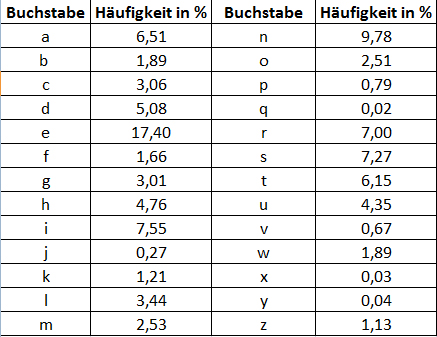
\includegraphics[width=260pt,height=200pt]{buchstaben-haeufigkeit-deutsches-alphabet.jpg}
\captionof{table}{Häufigkeit der Buchstaben in der deutschen Sprache \cite{Lindner2012}}
\end{table}
Dabei ist zu beachten, dass die Häufigkeitsanalyse aus mathematischen Gründen nur bei ausreichend langen Texten sicher funktioniert. In unserem Programm benötigt der eingegebene Text deshalb mindestens 26 Buchstaben.

\newpage

\subsection*{C++-Programm zur Ent-/Verschlüsselung}

\subsubsection*{Die Verschlüsselungsfunktion: encrypt\_text() in der Datei encrypt.cc}

Die Funktion nimmt als Argument einen zu verschlüsselnden Text, wobei der eingegebene Text mindestens 25 Zeichen enthalten muss, damit sich der Text auch wieder mit einer Häufigkeitsanalyse entschlüsseln lässt. Dann muss noch der Kleinbuchstabe eingegeben werden, auf den das a bei der Verschlüsselung abgebildet werden soll, um die Differenz c zu bestimmen. \\
Anschließend werden alle Großbuchstaben des Textes in Kleinbuchstaben umgewandelt. Dann wird über den ganzen Text iteriert und auf jeden Buchstaben die Verschlüsselungsfunktion C(x) angewandt, wobei Sonderzeichen nicht verschlüsselt werden, sondern einfach an der richtigen Stelle im Text wieder eingefügt werden. \\
Der verschlüsselte Text wird dann als string zurückgegeben.


\subsubsection*{Die Entschlüsselungsfunktion: decrypt\_text() in der Datei decrypt.cc}

Die Funktion nimmt einen Caesar-verschlüsselten Text als Eingabe, der mindestens die Länge 26 hat. Dann wird die Häufigkeit jedes Buchstaben im Text gezählt und in eine Priority Queue eingefügt, wobei der key die absolute Häufigkeit als integer ist und der value der entsprechende Buchstabe.\\
Der am häufigsten verwendete Buchstabe im verschlüsselten Text entspricht dann dem value des obersten Elements in der Priority Queue und kann einfach ausgelesen werden. Daraus kann die Differenz c wie oben beschrieben berechnet werden und anschließend die Funktion D(x) auf den gesamten Text angewendet werden.\\
Am Ende werden die ersten 30 Buchstaben des entschlüsselten Textes ausgegeben und überprüft, ob das wirklich der entschlüsselte Text ist.
Falls nicht, wird angenommen, dass der nächst häufigste Buchstabe das e war und der Text wird damit entschlüsselt. Das wird dreimal wiederholt, wenn dann kein richtiger Text gefunden wurde, kann angenommen werden, dass der eingegebene Text gar nicht Caesar-verschlüsselt war.\\
Entsprechen die ersten 30 Buchstaben einem korrekten Text, wird der ganze entschlüsselte Text als string zurückgegeben.

\subsubsection*{Demonstrationsfunktion: demo\_module() in der Datei demonstration.cc}

Die Funktion demo\_module nimmt einen Text als Eingabe und zeigt einmal die Verschlüsselung und Entschlüsselung. Die Funktion dient nur zur einfacheren Präsentation des Programms.\\
Auf den Text wird einmal die Funktion encrypt\_text angewendet und der verschlüsselte Text ausgegeben. Dann wird auf den verschlüsselten Text die Entschlüsselungsfunktion decrypt\_text angewendet und der Text wieder ausgegeben.

\subsubsection*{Formatierungsfunktion: format\_for\_print() in der Datei format\_print.cc}

Durch die Funktion format\_for\_print kann die Ausgabe von Texten in der Konsole schöner dargestellt werden. Das erleichtert die Nutzung auch bei kleineren Konsolenfenstern.

\subsubsection*{main\_program.cc}

Das main\_programm ist als einzige Datei zur Ausführung gedacht. Beim Ausführen wird abgefragt, welche der vier Optionen Verschlüsseln, Entschlüsseln eines Textes, Demonstration der Funktionen oder Beenden des Programms gewählt werden soll. Damit wird hier der gesamte Programmablauf koordiniert, die eigentliche Logik passiert aber an einer anderen Stelle.

\newpage
\listoftables
\printbibliography
\end{document} 